\documentclass[]{beamer}
%for printing or having a crappy pdf reader backup
%\documentclass[handout]{beamer}
\mode<presentation>
\usetheme{Madrid}


\usecolortheme[RGB={80,0,0}]{structure}
%teal \usecolortheme[RGB={0,128,128}]{structure}
\useoutertheme{miniframes}
\useinnertheme{default}
\usepackage{color}
\definecolor{Maroon}{RGB}{80,0,0}
\definecolor{BurntOrange}{RGB}{204,85,0}
\usepackage{setspace}
\usepackage{amsmath}
\usepackage{amsthm}
\usepackage{amsfonts}
\usepackage{amssymb}
\usepackage{verbatim}
\usepackage{array}
\usepackage{graphicx}
\usepackage{subfigure}
\usepackage{colortbl}
%\usepackage[retainorgcmds]{IEEEtrantools}
\usepackage{wrapfig}
\usepackage[figurename=,tablename=]{caption}
\usepackage{multirow}
\setbeamercolor{normal text}{fg=black}
\setbeamercovered{dynamic}
\beamertemplatetransparentcovereddynamicmedium
%\usepackage{chronology}
\setbeamertemplate{caption}[numbered]
\usepackage{colortbl}
\newcommand {\mathsym}[1]{{}}
\newcommand {\unicode}{{}}
\newcommand{\om}{\boldsymbol{\Omega}}
\newcommand{\etal}{{\it et al.\,}}
\newcommand{\vr}{\vec{r}}
\newcommand{\vo}{\vec{\Omega}}
\newcolumntype{L}{>{\centering\arraybackslash}m{3cm}}
\newcommand{\tcr}[1]{\textcolor{red}{#1}}
%Creating a norm command
\newcommand{\norm}[1]{\left\lVert#1\right\rVert}
%Allow page breaks within align
\allowdisplaybreaks
%Code
\usepackage{listings}
\usepackage{pdfpages}
\newlength \figwidth
\setlength \figwidth {0.5\textwidth}

\usepackage[percent]{overpic}



\begin{document}
%	

\title[XFEM Moving Interface Verification]{Extended Finite Element Method Development \& Application for Simulation of Moving Interface \& Boundary Phenomena}
\author[Tompkins]{James B. Tompkins \\ Chair: Dr. Ryan G. McClarren \\ Co-chair: Dr. Jean C. Ragusa \\ Committee: Drs. J.N. Reddy \& Lin Shao}
\institute[TAMU]{Texas A\&M University}
%\committee[McClarren,Arroyave,Ragusa,Shao,Hales]{Dr. Ryan McClarren \\ Dr. Raymundo Arr\'{o}yave \\ Dr. Jean Ragusa \\ Dr. Lin Shao \\ Dr. Jason Hales}
\date[Sept 6, 2018]

% ###############################################################################
\section{1D RZ LS Dep}
\subsection{}
% ###############################################################################
\begin{frame}[t]\frametitle{1D, Cylindrical, Level Set Dependent Material Problem Description}
  \begin{block}{PDE}
    $\rho c_p\frac{\partial T}{\partial t} - \nabla k \nabla T = \rho c_p\frac{\partial T}{\partial t} - \frac{1}{r} \frac{\partial}{\partial r}\left(r\cdot k \frac{\partial T}{\partial r} \right) = q$
  \end{block}
  
  \begin{block}{Domain/Material Properties}
  	$\Omega_r = [1,2], \,\,\ \rho c_p = 10, \,\, k=\left(\frac{0.05}{2.04}\right) \phi(x,t) + 1.5
  	= \frac{0.05}{2.04}\left( - x - 0.2t\right) + 1.55$
  \end{block}
  
  \begin{block}{BCs}
    Left:  \textbf{Neumann} -- $\left. \frac{\partial T}{\partial r}\right|_{r=1} = k(r,t) \cdot 200t$ \\
    Right: \textbf{Dirichlet} -- $T(2,t) = 400$
  \end{block}
  
  \begin{block}{ICs}
    \textbf{Constant} -- $T(r,0) = 400$
  \end{block}
\end{frame}

\begin{frame}[t]\frametitle{Method of Manufactured Solutions for 1D, RZ, LS Dependent Material Problem}
  \begin{block}{Prescribed Solution}
    $T(r,t) = (-200r+400)t + 400$
  \end{block}
  
  \begin{block}{Derived Source}
  $q = 200\,\rho c_p \left(-x+2\right) + \frac{1}{r}\left( 310t - \frac{10rt}{1.02} - \frac{t^2}{1.02}\right)$
  \end{block}
  
  \begin{block}{Interface Level Set Function}
    $\phi(r,t) = 2 - (r - 0.04) - 0.2t = 2.04 - r - 0.2t$
  \end{block}
\end{frame}

\begin{frame}\frametitle{Numerical Parameters}
  	\begin{columns}
		\column{0.32\linewidth}
			\begin{center}
			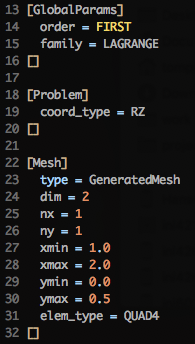
\includegraphics[scale=0.4]{figures/Screen-GlobalParams-1Drzls1m}
			\end{center}
		\column{0.66\linewidth}
			\begin{center}
			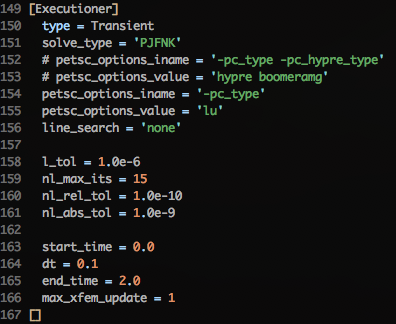
\includegraphics[scale=0.4]{figures/Screen-Executioner-1Drzls1m}
			\end{center}
	\end{columns}
	\begin{center}
	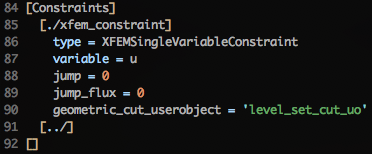
\includegraphics[scale=0.4]{figures/Screen-Constraints-1Drzls1m}
	\end{center}
\end{frame}

\begin{frame}[t]\frametitle{Results Comparison}
  	\begin{columns}
		\column{0.48\linewidth}
			\begin{center}
			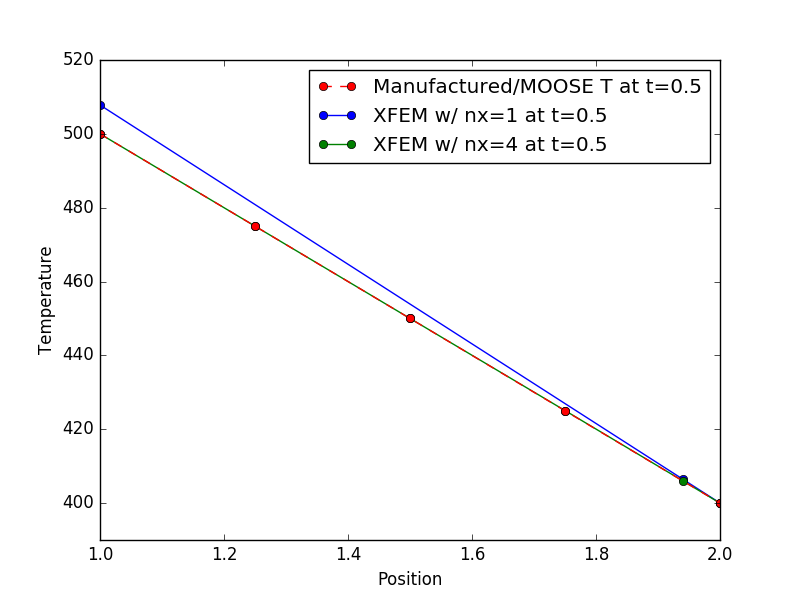
\includegraphics[scale=0.17]{figures/1D_rz_ls1mat_u_vs_x_05}\\
			$t=0.5$
			
			\null
			
			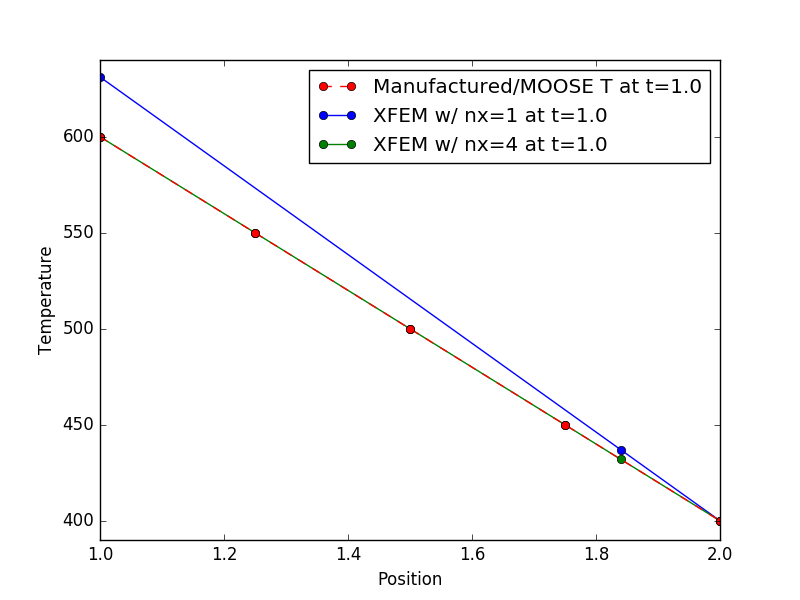
\includegraphics[scale=0.17]{figures/1D_rz_ls1mat_u_vs_x_10}\\
			$t=1.0$
			\end{center}
		\column{0.48\linewidth}
			\begin{center}
			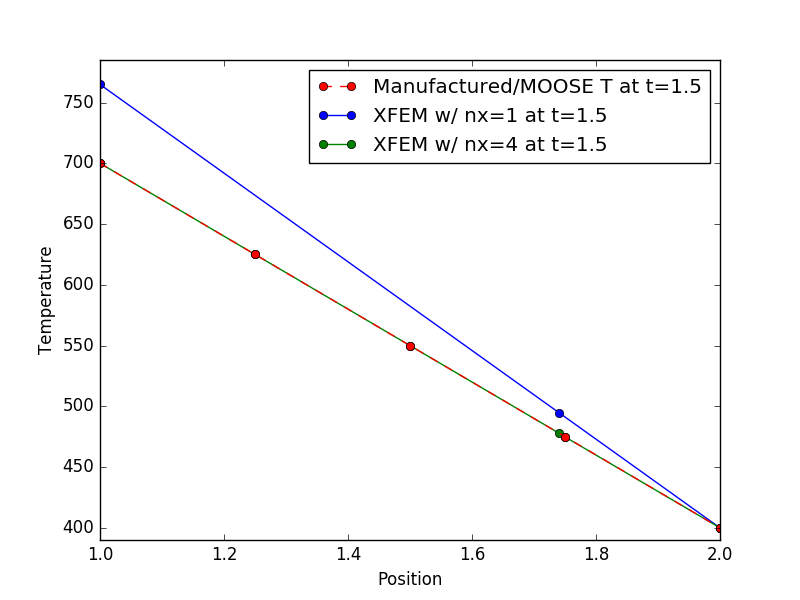
\includegraphics[scale=0.17]{figures/1D_rz_ls1mat_u_vs_x_15}\\
			$t=1.5$			
			
			\null
			
			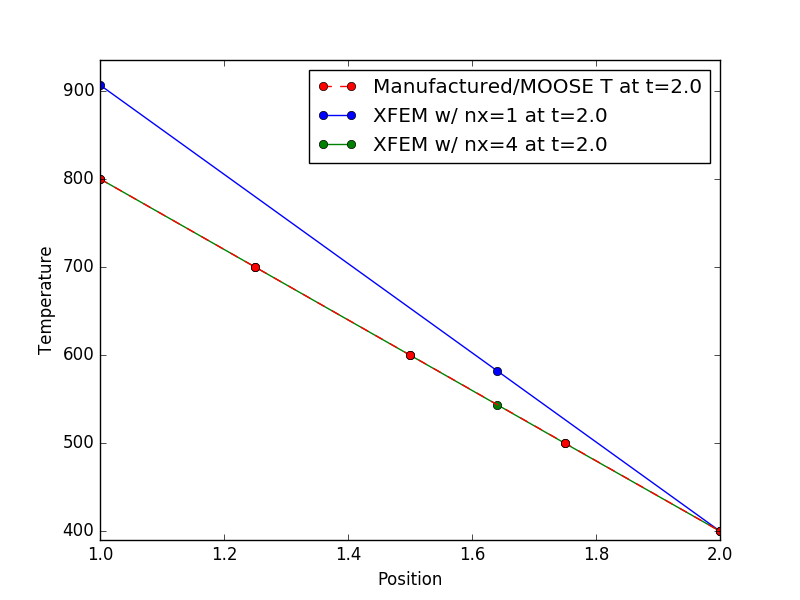
\includegraphics[scale=0.17]{figures/1D_rz_ls1mat_u_vs_x_20}\\
			$t=2.0$
			\end{center}
	\end{columns}
\end{frame}

\begin{frame}[t]\frametitle{L2 Error Norms at Each Timestep}
  	\begin{columns}
		\column{0.5\linewidth}
			\begin{center}
			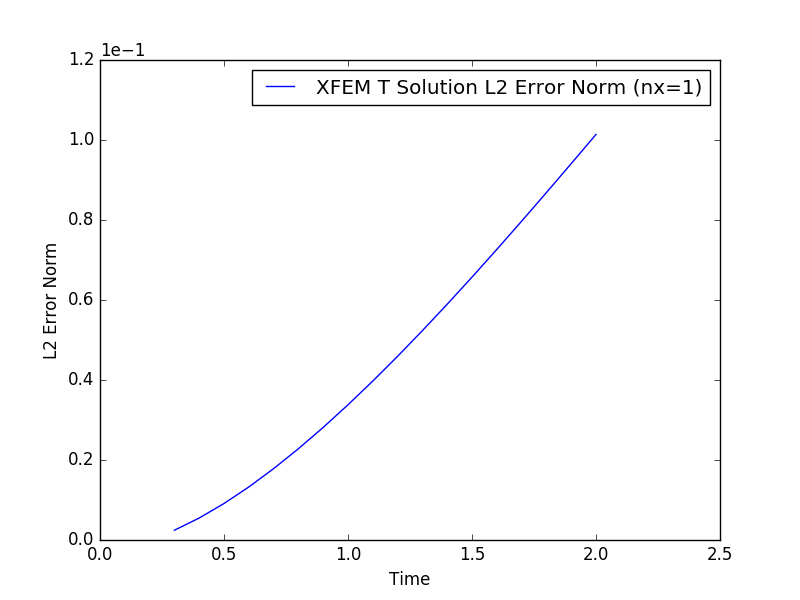
\includegraphics[scale=0.3]{figures/1D_rz_ls1mat_nx1_L2_Errs}
			\end{center}
		\column{0.5\linewidth}
			\begin{center}
			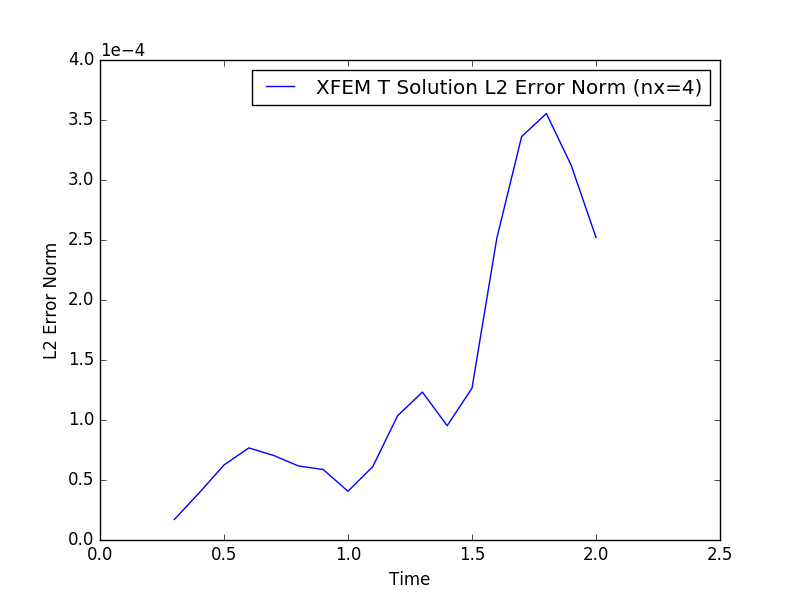
\includegraphics[scale=0.3]{figures/1D_rz_ls1mat_nx4_L2_Errs}
			\end{center}
	\end{columns}
\end{frame}

\begin{frame}[t]\frametitle{Mesh Refinement Effects on Error at x=1}
	\begin{center}
		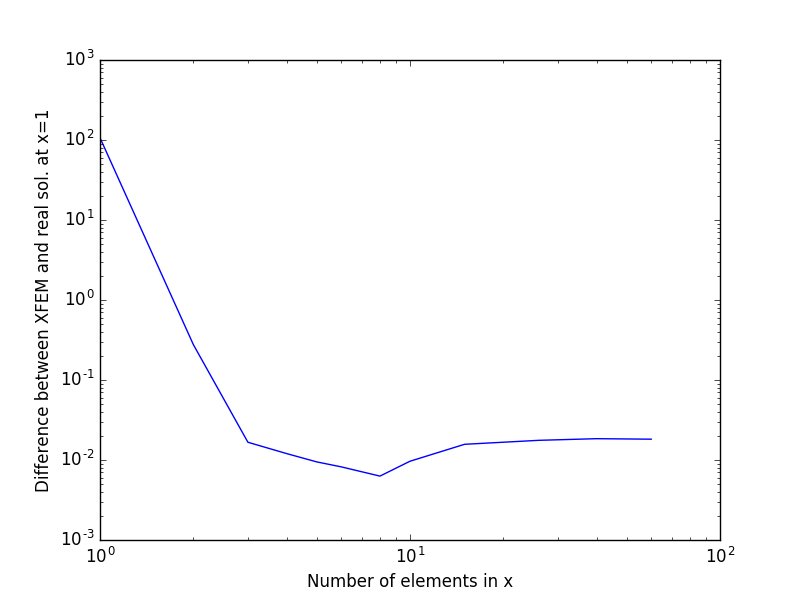
\includegraphics[scale=0.4]{figures/1D_rz_ls1mat_neumann_comp}
	\end{center}
\end{frame}

\end{document}

%%% Slide template
%\begin{frame}[t]\frametitle{}
%% Slide Goal: 
%% Notes: 
%  \begin{block}{}
%
%  \end{block}
%\end{frame}